% Architecture benchmark: the ablation study repeated on four architectures.
% Every number here comes from results/*.csv and the generated tables
% (scripts/analyze_models.py, scripts/collect_benchmark.py).

\section{Architecture benchmark}
\label{sec:benchmark}

\subsection{Setup}
The ablations of Section~\ref{sec:ablations} were run on DenseNet121 only, so they could not tell whether their conclusions belong to that network or to the task. We therefore repeated the same study on four ImageNet-pretrained architectures from \texttt{torchvision} that span a wide range of size and design:
DenseNet121~\cite{huang2017densenet} (7.0M parameters), ResNet50~\cite{he2016resnet} (23.5M), EfficientNet-B0~\cite{tan2019efficientnet} (4.0M) and ConvNeXt-Tiny~\cite{liu2022convnext} (27.8M).
For each one we trained three variants: fine-tuned with plain BCE, fine-tuned with the weighted BCE of Section~\ref{sec:ablations}, and a frozen backbone where only the new 14-way head is trained. DenseNet121 was trained with two extra seeds for both fine-tuned variants, giving \textbf{16 training runs}.

Everything else is identical across runs: the patient-wise split, $224\times224$ inputs with a random horizontal flip, Adam with learning rate $10^{-4}$, batch size 32, 5 epochs, mixed precision, seed 0 unless stated, and the checkpoint with the best validation mean AUC. Each run then predicts the validation and test sets and scores its Grad-CAM heatmaps (Section~\ref{sec:localisation}) in the same Kaggle job, so no number is copied between scripts by hand.

\paragraph{Making 16 runs affordable.} Decoding the 1024-pixel PNGs, not the GPU, was the bottleneck (30--45 minutes per epoch). Each job now decodes every image once into a $224\times224$ 8-bit cache (about 19 minutes for 112{,}120 images, 5.6\,GB), after which an epoch takes about 8 minutes. The cache stores exactly the output of the resize used by the transforms, so training sees the same tensors; the DenseNet121 plain-BCE run reproduces the earlier ablation (validation 0.833 against 0.836, within the seed-to-seed spread measured below).

\paragraph{Statistics.} Test AUCs come with a 95\% confidence interval from a bootstrap that resamples \emph{patients} (1{,}000 resamples), because images of one patient are not independent. Two models are compared with a \emph{paired} bootstrap on the same resamples, which gives an interval and a p-value for their difference; with 1{,}000 resamples the smallest p-value it can resolve is 0.002. This captures the uncertainty due to the finite test set, not the randomness of training; the extra DenseNet121 seeds measure the latter.

\subsection{The same study on every architecture}
\begin{figure}[ht]
\centering
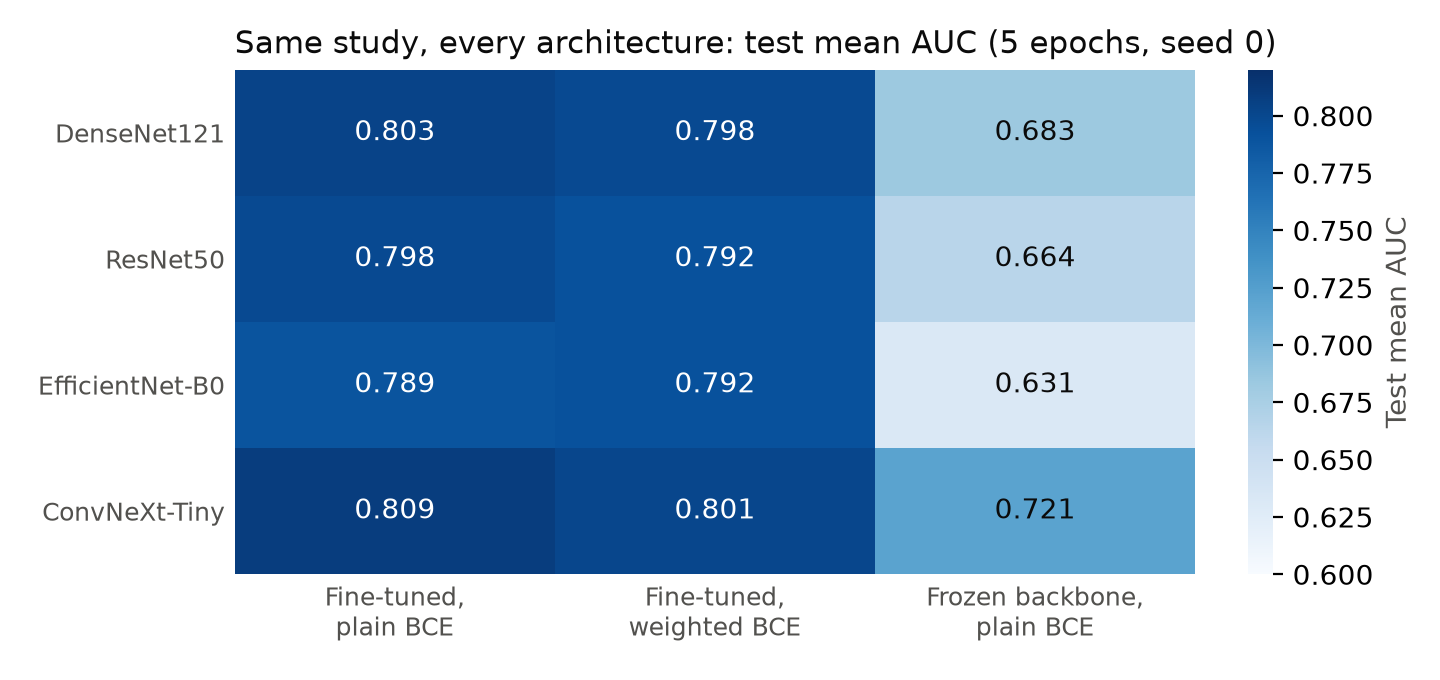
\includegraphics[width=0.82\textwidth]{grid_heatmap.png}
\caption{Test mean AUC for every architecture and variant (seed 0). The full table with confidence intervals is Table~\ref{tab:grid}.}
\label{fig:grid}
\end{figure}

\begin{table}[ht]
\centering\small
\resizebox{\textwidth}{!}{\begin{tabular}{lccc}
\toprule
Architecture & Fine-tuned, plain BCE & Fine-tuned, weighted BCE & Frozen backbone, plain BCE \\
\midrule
DenseNet121 & 0.803 [0.796, 0.808] & 0.798 [0.791, 0.803] & 0.683 [0.675, 0.691] \\
ResNet50 & 0.798 [0.791, 0.804] & 0.792 [0.785, 0.798] & 0.664 [0.655, 0.672] \\
EfficientNet-B0 & 0.789 [0.782, 0.795] & 0.792 [0.785, 0.798] & 0.631 [0.623, 0.639] \\
ConvNeXt-Tiny & \textbf{0.809 [0.802, 0.814]} & \textbf{0.801 [0.793, 0.808]} & \textbf{0.721 [0.713, 0.728]} \\
\bottomrule
\end{tabular}
}
\caption{Test mean AUC [95\% patient-bootstrap CI], official test split (25{,}596 images). Bold: best architecture in each column.}
\label{tab:grid}
\end{table}

Figure~\ref{fig:grid} and Table~\ref{tab:grid} answer the question the DenseNet ablations left open.

\paragraph{Fine-tuning matters for every architecture.} Freezing the backbone costs between 0.088 (ConvNeXt-Tiny) and 0.158 (EfficientNet-B0) of test AUC. ImageNet features are not enough for chest X-rays, whatever the network.

\paragraph{Class weighting does not help, on three architectures out of four.} The weighted loss lowers test AUC for DenseNet121 ($-0.005$, 95\% CI $[-0.009,-0.001]$, $p=0.008$), ResNet50 ($-0.006$, $[-0.010,-0.002]$, $p=0.008$) and ConvNeXt-Tiny ($-0.008$, $[-0.012,-0.004]$, $p<0.002$). EfficientNet-B0 is the exception: weighted is $0.003$ higher, but the difference is not significant ($[-0.001, 0.008]$, $p=0.11$).

\begin{table}[ht]
\centering\small
\begin{tabular}{lccc}
\toprule
DenseNet121 & Seeds & Val AUC (mean $\pm$ sd) & Test AUC (mean $\pm$ sd) \\
\midrule
Fine-tuned, plain BCE & 3 & 0.8331 $\pm$ 0.0020 & 0.8056 $\pm$ 0.0024 \\
Fine-tuned, weighted BCE & 3 & 0.8190 $\pm$ 0.0013 & 0.7968 $\pm$ 0.0009 \\
\bottomrule
\end{tabular}

\caption{DenseNet121 trained three times with different seeds per loss.}
\label{tab:seeds}
\end{table}

\paragraph{The effect is larger than the seed-to-seed noise.} The first report called the 0.013 validation gap ``suggestive only'' because it came from one run per setting. With three seeds each (Table~\ref{tab:seeds}), every plain-BCE run (test 0.803, 0.807, 0.807) is above every weighted run (0.798, 0.796, 0.796). The mean gap, 0.009 on test, is about four times the standard deviation between seeds (0.002), so it is not a lucky seed.

\subsection{Which architecture, and at what cost}
\begin{figure}[ht]
\centering
\begin{minipage}{0.49\textwidth}\centering
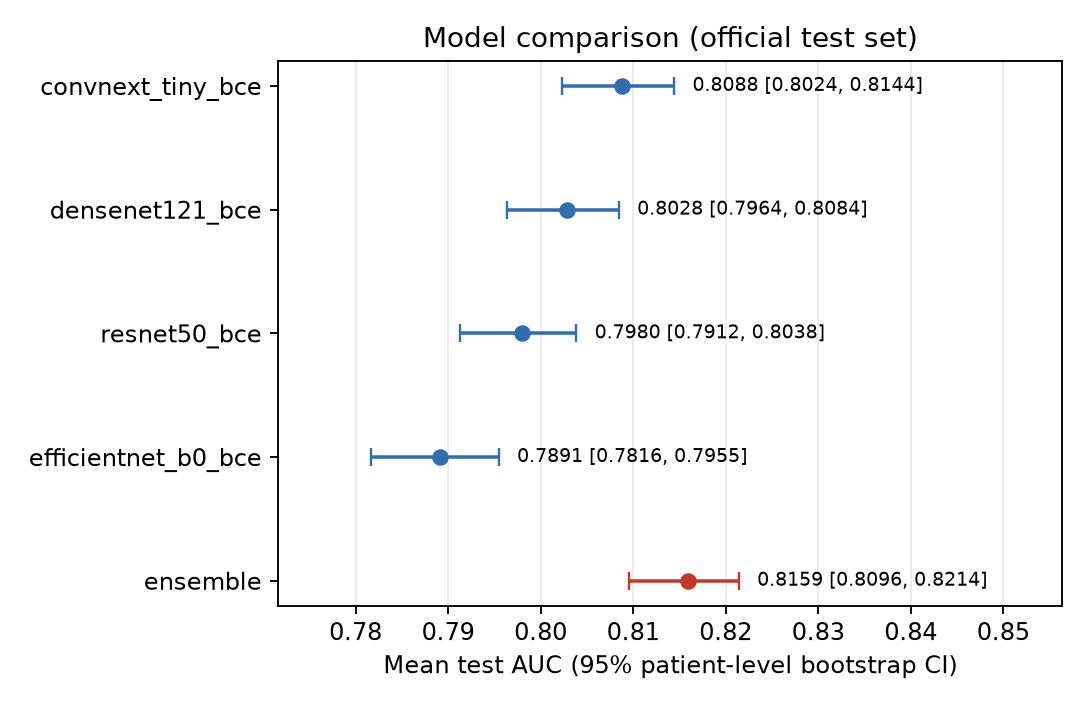
\includegraphics[width=\textwidth]{forest_auc.png}
\end{minipage}\hfill
\begin{minipage}{0.49\textwidth}\centering
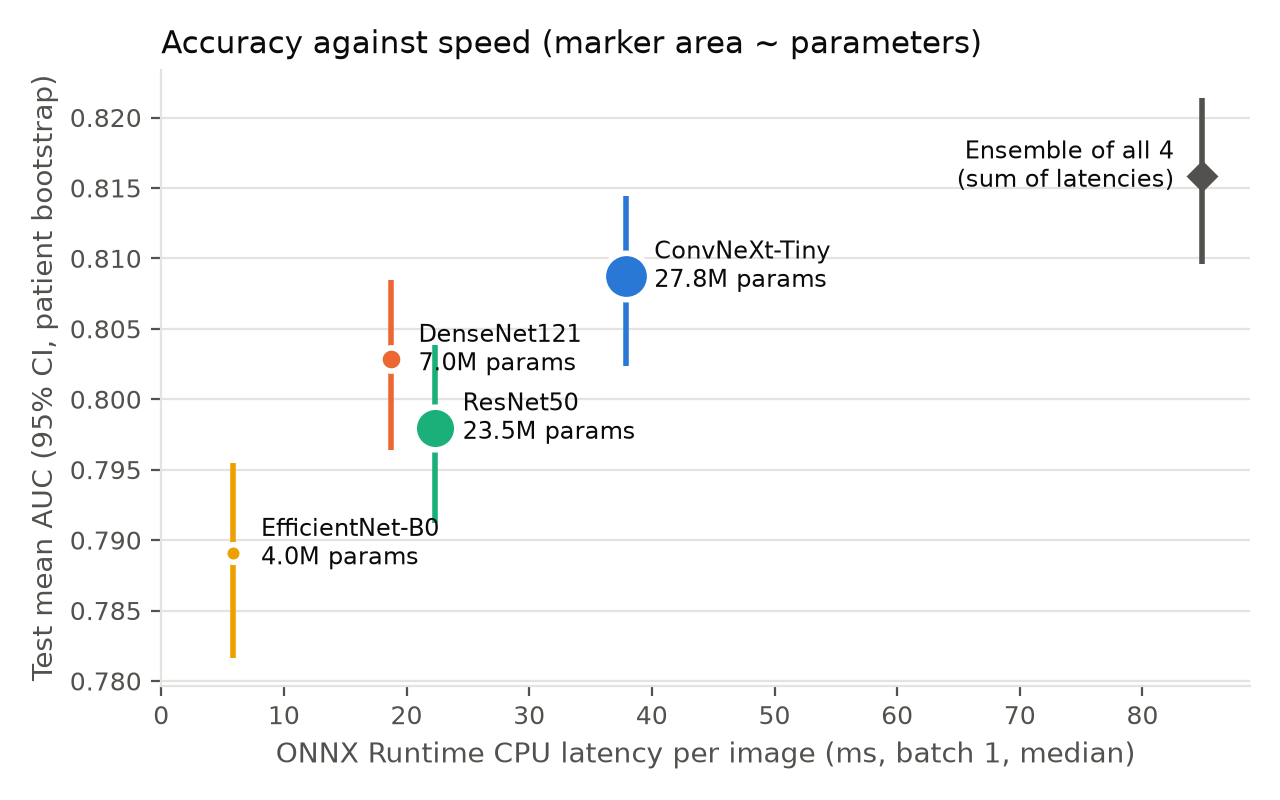
\includegraphics[width=\textwidth]{pareto.png}
\end{minipage}
\caption{Left: test mean AUC with 95\% CI for the plain-BCE models and their ensemble. Right: AUC against ONNX Runtime CPU latency per image (batch 1, median of 100 runs on a 16-thread laptop CPU); marker area is proportional to the number of parameters.}
\label{fig:forest}
\end{figure}

With the recipe fixed, ConvNeXt-Tiny is the most accurate single model (0.809 [0.802, 0.814]), followed by DenseNet121 (0.803), ResNet50 (0.798) and EfficientNet-B0 (0.789) (Figure~\ref{fig:forest}). The paired tests separate every pair (no bootstrap resample reverses any of the orders, $p<0.002$), but this needs care: ConvNeXt-Tiny is ahead of DenseNet121 by 0.006, and DenseNet121's own seeds range from 0.803 to 0.807. We did not train ConvNeXt-Tiny with several seeds, so its lead over DenseNet121 is likely but not established. Its lead over EfficientNet-B0 (0.020) is far outside that noise.

\paragraph{Ensemble.} Averaging the probabilities of the four plain-BCE models gives \textbf{0.816} [0.810, 0.821], above the best single model by 0.007 ([0.005, 0.009], $p<0.002$), a gain larger than the whole seed-to-seed range of DenseNet121. It also has the lowest calibration error (Table~\ref{tab:benchmark}). The cost is running four networks: about 85\,ms per image on CPU instead of 6--38\,ms.

\paragraph{Cost.} EfficientNet-B0 is 6.5 times faster than ConvNeXt-Tiny (5.9 against 37.9\,ms) for 0.020 less AUC; DenseNet121 (18.7\,ms) is a good middle point. Accuracy did not simply follow size: ResNet50 has 3.4 times more parameters than DenseNet121 and is less accurate.

\subsection{Calibration}
\label{sec:calibration_bench}
A temperature $T$ is fitted on the validation split for each model (minimising the BCE of $\sigma(z/T)$), and the expected calibration error (ECE, 15 bins, all classes pooled) is reported on test before and after (Table~\ref{tab:benchmark}, Figure~\ref{fig:calib_bench}). Dividing by $T$ does not change the ranking, so AUC is unchanged.

\begin{figure}[ht]
\centering
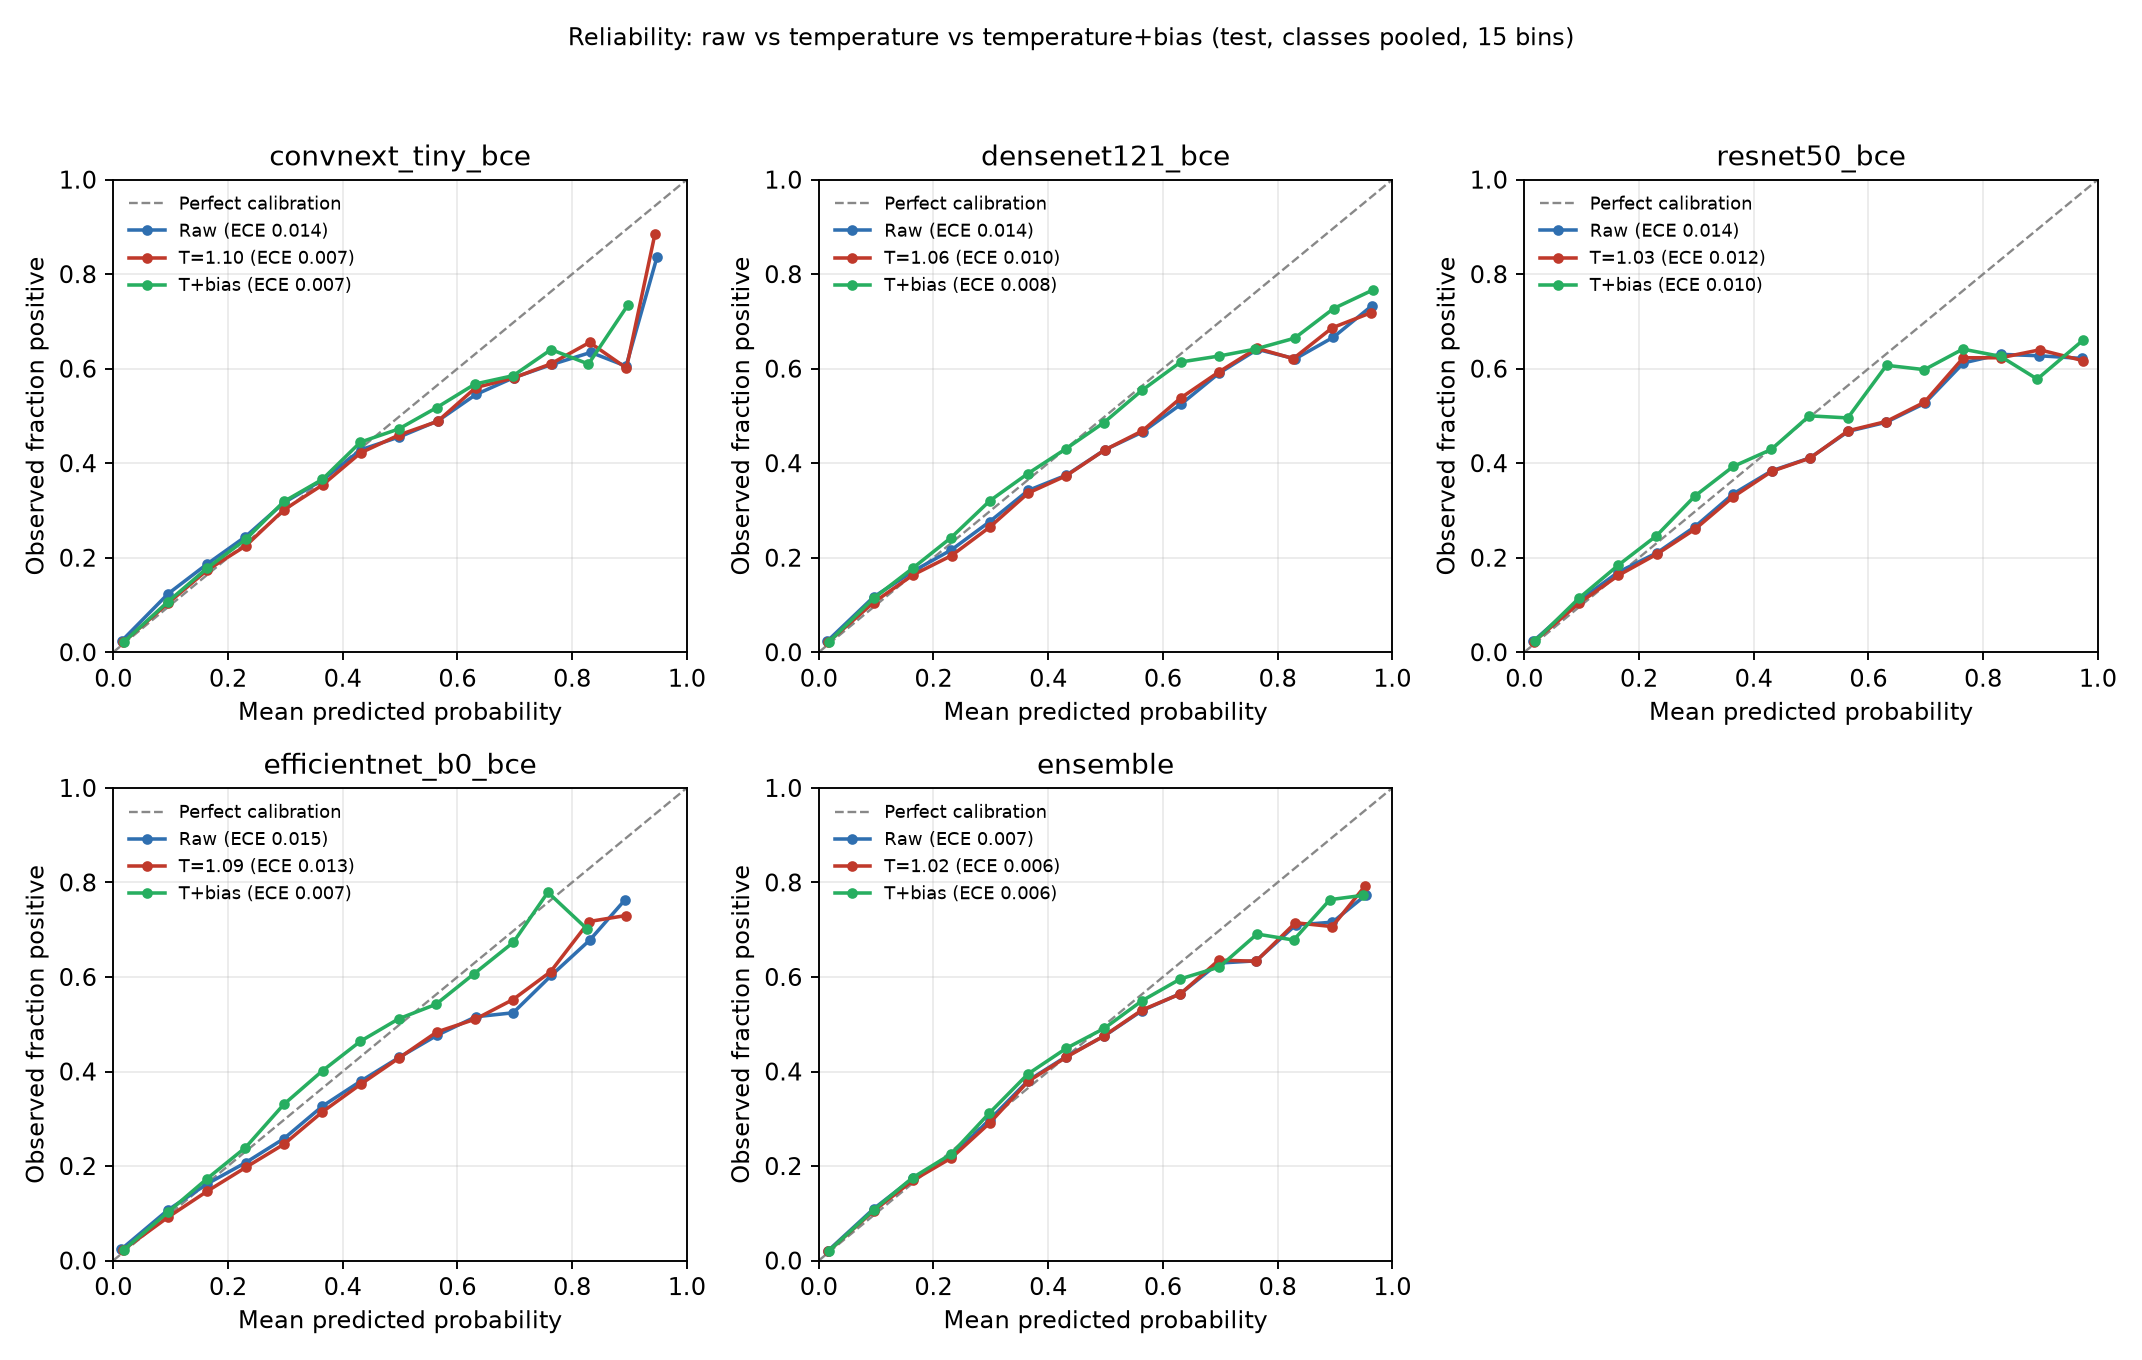
\includegraphics[width=0.95\textwidth]{calibration_before_after.png}
\caption{Reliability on the test set for the plain-BCE models: raw scores, after temperature scaling ($T$), and after temperature plus a bias term (Platt scaling), all fitted on validation.}
\label{fig:calib_bench}
\end{figure}

\paragraph{The over-confidence came from the weighted loss.} The four plain-BCE models are already close to calibrated (test ECE 0.014--0.015), and their fitted temperatures are close to 1 (1.03--1.10), lowering ECE to 0.007--0.013. Every weighted model is far off (ECE 0.33--0.36), which explains the over-confident scores of the original model (Figure~\ref{fig:calibration}). Temperature scaling cannot repair them (ECE stays at 0.33--0.36): the weights shift every logit upwards, and a scale factor cannot remove a shift. Adding a bias term (Platt scaling) does, bringing them to 0.009--0.018. The application therefore serves plain-BCE models with their temperatures, and the numbers it displays can be read as probabilities.

\subsection{Do the heatmaps point at the lesion?}
\label{sec:localisation}
The first report only showed heatmaps qualitatively. The NIH release includes 984 bounding boxes drawn by radiologists on 880 images for eight findings; none of these images is in our training split. For each box we compute the Grad-CAM heatmap of that finding (on the last convolutional block of each architecture) and measure:
\begin{itemize}
  \item the \textbf{pointing game}: whether the hottest point of the heatmap falls inside the box;
  \item the \textbf{energy}: the share of the heatmap's total mass inside the box;
  \item the \textbf{IoU} between the box and the region where the heatmap is at least half its maximum.
\end{itemize}
Two references need no model: a point placed at random lands in the box 7.8\% of the time (the mean box area), and a point always at the image centre lands in it 21.8\% of the time.

\begin{figure}[ht]
\centering
\begin{minipage}{0.49\textwidth}\centering
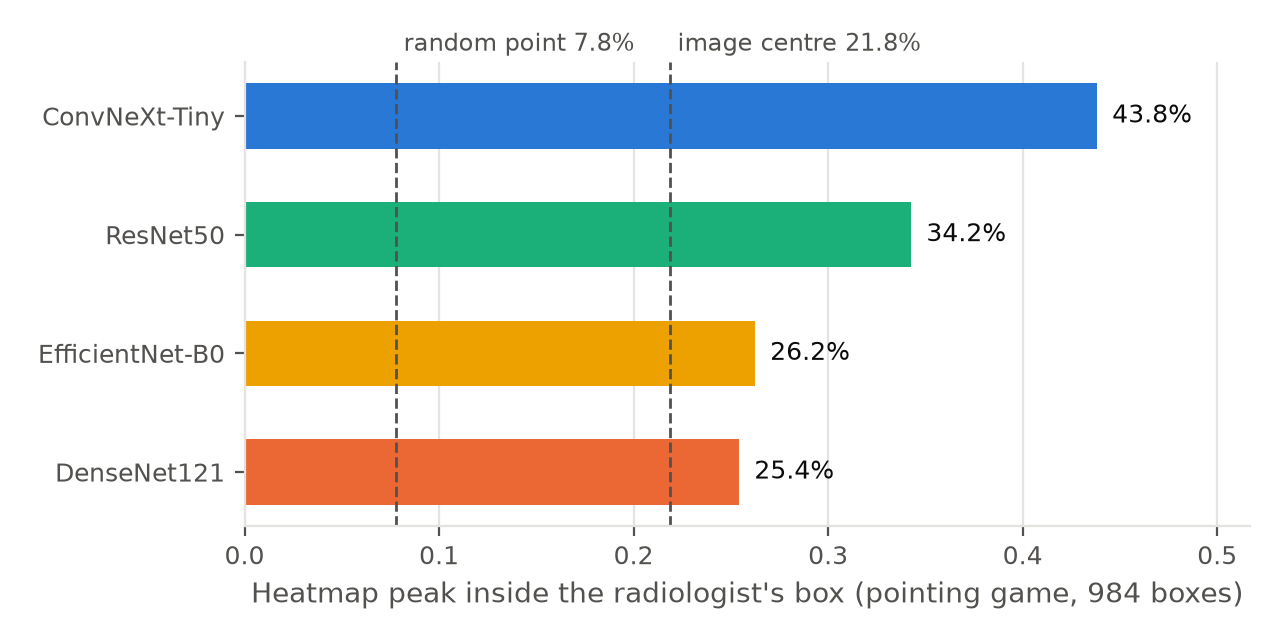
\includegraphics[width=\textwidth]{localization_bars.png}
\end{minipage}\hfill
\begin{minipage}{0.49\textwidth}\centering
\begin{tabular}{lccc}
\toprule
Model & Pointing game (hit) & Energy in box & IoU (heat $\geq$ 0.5) \\
\midrule
ConvNeXt-Tiny & 0.438 & 0.299 & 0.178 \\
ResNet50 & 0.342 & 0.227 & 0.127 \\
EfficientNet-B0 & 0.262 & 0.117 & 0.135 \\
DenseNet121 & 0.254 & 0.176 & 0.145 \\
\midrule
Random point (baseline) & 0.078 & -- & -- \\
Image centre (baseline) & 0.218 & -- & -- \\
\bottomrule
\end{tabular}

\end{minipage}
\caption{Grad-CAM localisation of the plain-BCE models against the 984 expert boxes.}
\label{fig:localisation}
\end{figure}

\begin{figure}[ht]
\centering
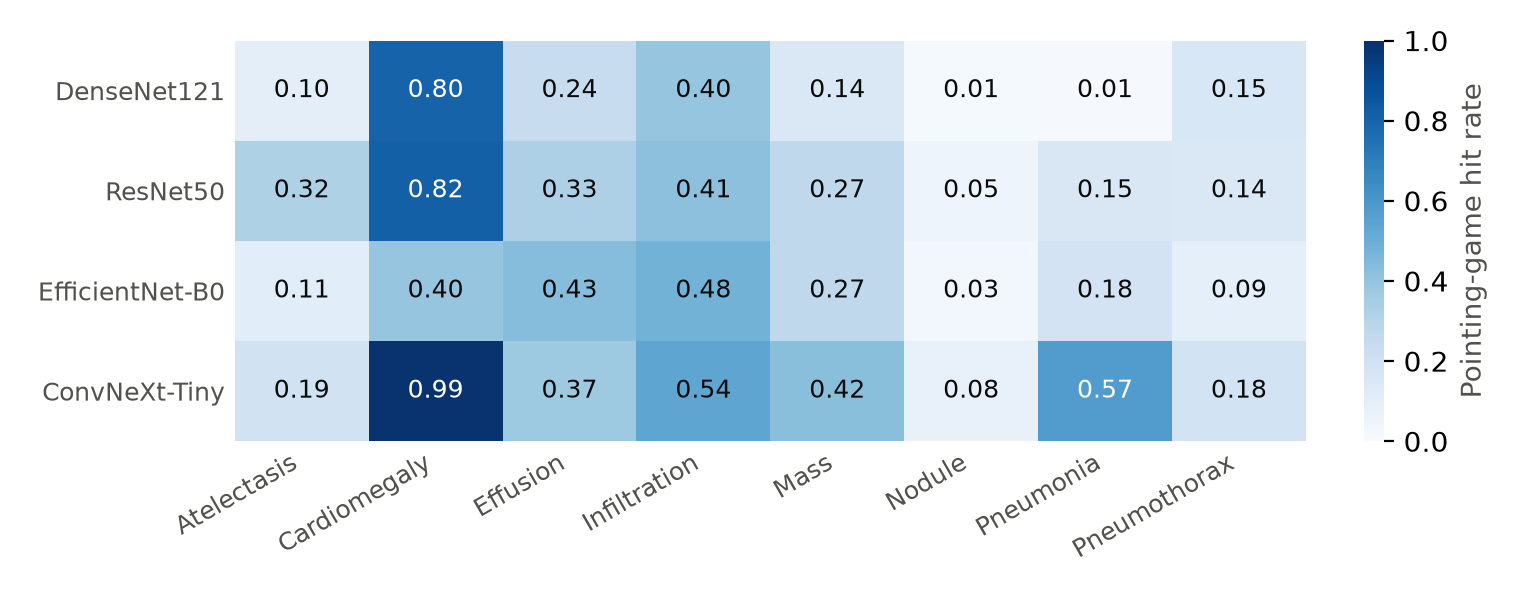
\includegraphics[width=0.85\textwidth]{localization_per_disease.png}
\caption{Pointing-game hit rate per finding. Nodule boxes cover 0.6\% of the image on average, smaller than one cell of the $7\times7$ feature map that Grad-CAM upsamples, so no model can localise them.}
\label{fig:localisation_disease}
\end{figure}

\paragraph{Results.} ConvNeXt-Tiny puts its peak inside the box for 43.8\% of the boxes, twice the centre baseline, and is also best on energy and IoU (Figure~\ref{fig:localisation}). ResNet50 follows (34.2\%). DenseNet121 (25.4\%) and EfficientNet-B0 (26.2\%) are only slightly better than always pointing at the centre. So the most accurate classifier is also the one whose explanations are most often right, but a good AUC does not by itself imply good heatmaps.

The findings differ sharply (Figure~\ref{fig:localisation_disease}). Cardiomegaly, whose box is the heart, is localised by every model except EfficientNet-B0 (ConvNeXt-Tiny 0.99). Nodules are never localised (at most 0.08), as the caption explains. For Pneumonia, ConvNeXt-Tiny points into the box 57\% of the time and DenseNet121 1\%.

\paragraph{Caveats.} These numbers are noisier than the AUCs: the three DenseNet121 plain-BCE seeds give 25.4\%, 27.0\% and 32.5\%, so only large differences such as ConvNeXt-Tiny's lead should be trusted. Two observations are consistent but unexplained: the weighted-loss models localise as well as or better than their plain counterparts (ResNet50 40.0\% against 34.2\%, EfficientNet-B0 42.6\% against 26.2\%) despite their lower AUC, and frozen backbones localise worse than the centre baseline (11.5--12.5\%). The frozen ResNet50 and EfficientNet-B0 runs have no localisation score: Grad-CAM failed on frozen backbones in those two jobs, a bug fixed before the other frozen runs, and the saved predictions were kept.

\subsection{Subgroups}
\begin{figure}[ht]
\centering
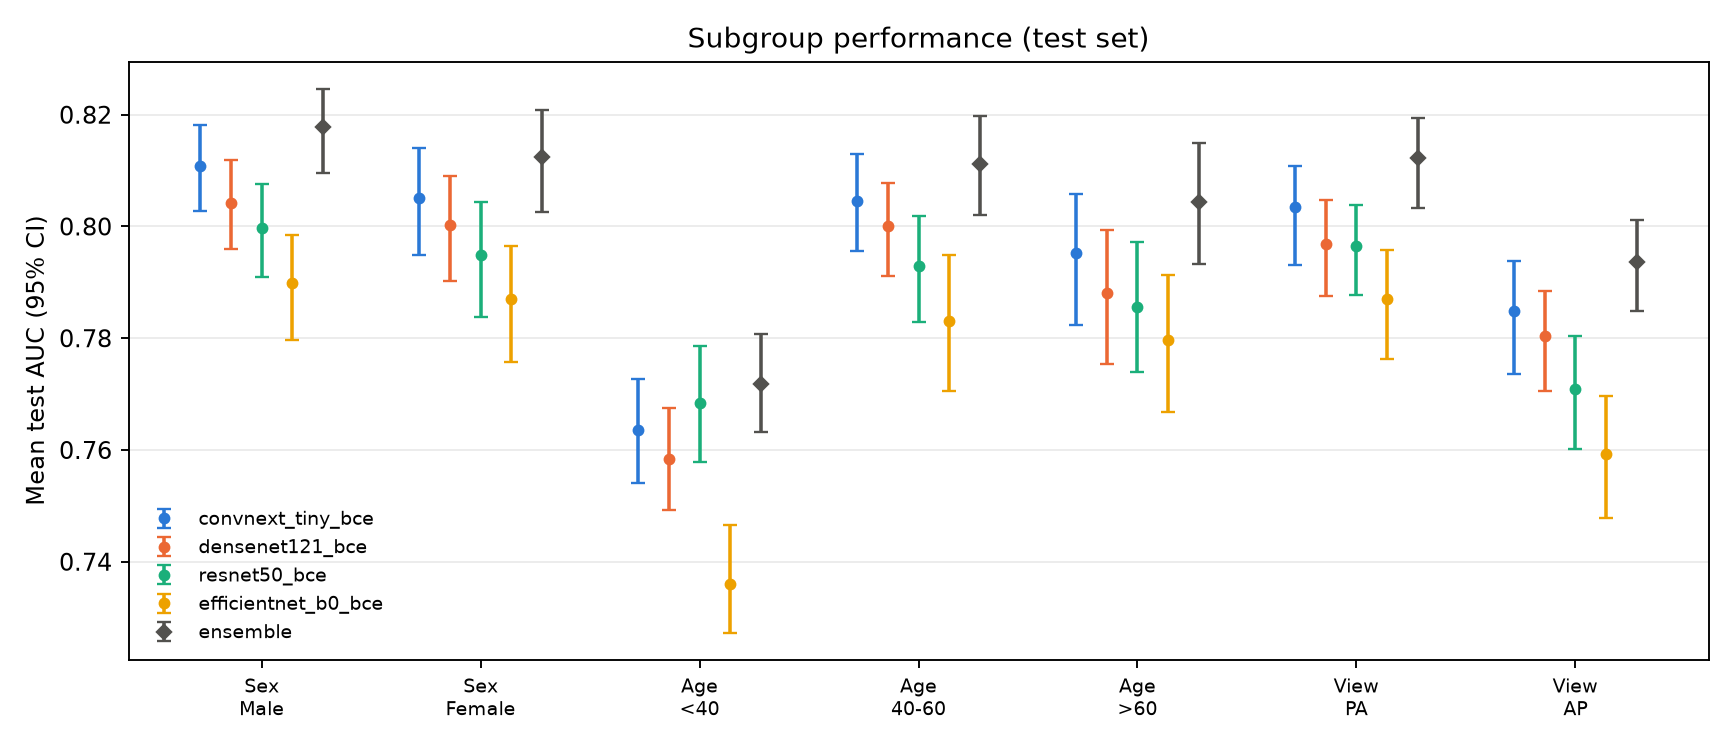
\includegraphics[width=0.95\textwidth]{subgroups.png}
\caption{Test mean AUC with 95\% CI by sex, age and view position, from the metadata of the NIH release.}
\label{fig:subgroups}
\end{figure}

\begin{table}[ht]
\centering\small
\resizebox{\textwidth}{!}{\begin{tabular}{ll rccccc}
\toprule
Group & Level & $n$ & convnext\_tiny\_bce & densenet121\_bce & resnet50\_bce & efficientnet\_b0\_bce & ensemble \\
\midrule
Sex & Male & 14,882 & 0.811 [0.803, 0.818] & 0.804 [0.796, 0.812] & 0.800 [0.791, 0.808] & 0.790 [0.780, 0.798] & 0.818 [0.810, 0.825] \\
Sex & Female & 10,714 & 0.805 [0.795, 0.814] & 0.800 [0.790, 0.809] & 0.795 [0.784, 0.804] & 0.787 [0.776, 0.797] & 0.813 [0.803, 0.821] \\
Age & <40 & 8,290 & 0.764 [0.754, 0.773] & 0.758 [0.749, 0.767] & 0.768 [0.758, 0.779] & 0.736 [0.727, 0.747] & 0.772 [0.763, 0.781] \\
Age & 40-60 & 11,733 & 0.805 [0.796, 0.813] & 0.800 [0.791, 0.808] & 0.793 [0.783, 0.802] & 0.783 [0.771, 0.795] & 0.811 [0.802, 0.820] \\
Age & >60 & 5,573 & 0.795 [0.782, 0.806] & 0.788 [0.775, 0.799] & 0.786 [0.774, 0.797] & 0.780 [0.767, 0.791] & 0.804 [0.793, 0.815] \\
View & PA & 11,096 & 0.803 [0.793, 0.811] & 0.797 [0.788, 0.805] & 0.797 [0.788, 0.804] & 0.787 [0.776, 0.796] & 0.812 [0.803, 0.819] \\
View & AP & 14,500 & 0.785 [0.774, 0.794] & 0.780 [0.771, 0.788] & 0.771 [0.760, 0.780] & 0.759 [0.748, 0.770] & 0.794 [0.785, 0.801] \\
\bottomrule
\end{tabular}
}
\caption{Subgroup test mean AUC [95\% CI]. $n$ is the number of test images in the group.}
\label{tab:subgroups}
\end{table}

All models behave the same way across subgroups (Figure~\ref{fig:subgroups}, Table~\ref{tab:subgroups}). There is no gap between men and women. Two gaps are clear and shared by every architecture:
\begin{itemize}
  \item patients under 40 are harder (ConvNeXt-Tiny 0.764 against 0.805 for 40--60);
  \item AP films are harder than PA films (0.785 against 0.803). AP films are usually taken at the bedside, on patients too ill to stand, with more overlapping devices and lower image quality.
\end{itemize}
We report these gaps but cannot separate their causes, such as different disease mixes per group and label noise, with the data available.

\subsection{Full results}
\begin{table}[ht]
\centering
\resizebox{\textwidth}{!}{\begin{tabular}{lcrrrrrrr}
\toprule
Model & Mean AUC [95\% CI] & AP & ECE & ECE (T) & $T$ & ECE (T+b) & Params & Latency (ms) \\
\midrule
convnext\_tiny\_bce & 0.8088 [0.802, 0.814] & 0.276 & 0.014 & 0.007 & 1.10 & 0.007 & 27.8M & 37.9 \\
convnext\_tiny\_frozen & 0.7208 [0.713, 0.728] & 0.156 & 0.013 & 0.012 & 1.01 & 0.012 & 27.8M & -- \\
convnext\_tiny\_weighted & 0.8011 [0.793, 0.808] & 0.267 & 0.336 & 0.339 & 1.11 & 0.009 & 27.8M & -- \\
densenet121\_bce & 0.8028 [0.796, 0.808] & 0.259 & 0.014 & 0.010 & 1.06 & 0.008 & 7.0M & 18.7 \\
densenet121\_bce\_s1 & 0.8067 [0.800, 0.812] & 0.279 & 0.016 & 0.014 & 1.06 & 0.007 & 7.0M & -- \\
densenet121\_bce\_s2 & 0.8071 [0.801, 0.812] & 0.276 & 0.009 & 0.009 & 1.00 & 0.006 & 7.0M & -- \\
densenet121\_frozen & 0.6826 [0.675, 0.691] & 0.136 & 0.011 & 0.014 & 0.96 & 0.015 & 7.0M & -- \\
densenet121\_weighted & 0.7978 [0.791, 0.803] & 0.259 & 0.359 & 0.361 & 1.07 & 0.017 & 7.0M & -- \\
densenet121\_weighted\_s1 & 0.7963 [0.789, 0.802] & 0.264 & 0.338 & 0.337 & 0.96 & 0.011 & 7.0M & -- \\
densenet121\_weighted\_s2 & 0.7963 [0.789, 0.803] & 0.255 & 0.329 & 0.330 & 1.03 & 0.016 & 7.0M & -- \\
efficientnet\_b0\_bce & 0.7891 [0.782, 0.795] & 0.247 & 0.015 & 0.013 & 1.09 & 0.007 & 4.0M & 5.9 \\
efficientnet\_b0\_frozen & 0.6310 [0.623, 0.639] & 0.118 & 0.017 & 0.017 & 0.98 & 0.018 & -- & -- \\
efficientnet\_b0\_weighted & 0.7925 [0.785, 0.798] & 0.252 & 0.339 & 0.342 & 1.11 & 0.013 & 4.0M & -- \\
resnet50\_bce & 0.7980 [0.791, 0.804] & 0.252 & 0.014 & 0.012 & 1.03 & 0.010 & 23.5M & 22.3 \\
resnet50\_frozen & 0.6640 [0.655, 0.672] & 0.127 & 0.015 & 0.017 & 0.98 & 0.017 & -- & -- \\
resnet50\_weighted & 0.7920 [0.785, 0.798] & 0.256 & 0.329 & 0.333 & 1.15 & 0.011 & 23.5M & -- \\
\midrule
ensemble & \textbf{0.8159} [0.810, 0.821] & 0.283 & 0.007 & 0.006 & 1.02 & 0.006 & -- & -- \\
\bottomrule
\end{tabular}
}
\caption{All 16 runs and the ensemble on the test set: mean AUC [95\% CI], average precision, ECE raw / after temperature scaling / after temperature and bias, the fitted temperature, parameters and CPU latency (measured for the served models). Run names are \texttt{architecture\_variant[\_seed]}.}
\label{tab:benchmark}
\end{table}
